\documentclass{exam}
\usepackage{graphicx}
\usepackage[utf8]{inputenc}
\usepackage[english]{babel}
\usepackage{amsmath}
\usepackage{hyperref}
\usepackage{amsthm}
\usepackage{tcolorbox}
\usepackage{amsfonts}
\usepackage{amssymb}

\newbox\eeveebox
\setbox\eeveebox\hbox{
\raisebox{-2.5pt}{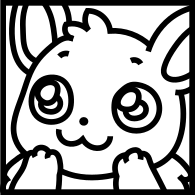
\includegraphics[height=2.5ex]{iibui.png}}}
\def\eeveeKawaii{\copy\eeveebox}

\NewTColorBox{proposition}{m}{
  standard jigsaw,
  sharp corners,
  boxrule=0.4pt,
  coltitle=black,
  colframe=black,
  opacityback=0,
  opacitybacktitle=0,
  fonttitle=\normalfont\bfseries\upshape,
  fontupper=\normalfont\itshape,
  title={Proposition #1},
  after title={.},
  attach title to upper={\ },
}

\renewcommand\qedsymbol{$\eeveeKawaii$}

\title{Hammack Exercises - Chapter 5}
\author{FungusDesu}
\date{September 1st 2024}

\begin{document}

\maketitle

\section{Preface}
i dont really have anything to say

\section{Section A - Contrapositive proof only}
\begin{proposition}{5.1}
    Suppose $n\in\mathbb Z$. If $n^2$ is even, then $n$ is even.
\end{proposition}

\begin{proof}
    We shall prove this statement via contrapositive proof. Suppose $n$ is odd; we wish to show that $n^2$ is odd. Then $n = 2k + 1$ for some $k\in\mathbb Z$. It follows that $n^2 = (2k + 1)^2 = 4k^2 + 4k + 1$, thus $n^2 = 2x + 1$ where $x = 2k^2 + 2k \in\mathbb Z$. Therefore $n^2$ is odd by definition of an odd number, as desired.
\end{proof}

\begin{proposition}{5.2}
    Suppose $n\in\mathbb Z$. If $n^2$ is odd, then $n$ is odd.
\end{proposition}

\begin{proof}
    We shall prove this statement via contrapositive proof. Suppose $n$ is even; we wish to show that $n^2$ is even. Then $n = 2k$ for some $k\in\mathbb Z$. It follows that $n^2 = (2k)^2 = 4k^2$, thus $n^2 = 2x$ where $x = 2k^2 \in\mathbb Z$. Therefore $n^2$ is even by definition of an even number, as desired.
\end{proof}

\begin{proposition}{5.3}
    Suppose $a, b\in\mathbb Z$. If $a^2(b^2-2b)$ is odd, then $a$ and $b$ are odd.
\end{proposition}

\begin{proof}
    We shall prove this statement via contrapositive proof. Suppose $a$ is even or $b$ is even; we wish to show that $a^2(b^2-2b)$ is even. We divide into two cases as follow
    \begin{description}
        \item[Case 1. ] If $a$ is even, then $a = 2k$ for some $k\in\mathbb Z$. It follows that \[
        (2k)^2(b^2-2b)=4k^2(b^2-2b)
        \]
        implying $a^2(b^2-2b) =2x$ where $x = 2k^2(b^2-2b) \in\mathbb Z$. Thus for all even $a$, the number $a^2(b^2-2b)$ is even.
        \item[Case 2. ] If $b$ is even, then $b = 2k$ for some $k\in\mathbb Z$. It follows that \[
        a^2((2k)^2-2(2k)) = a^2(4k^2-4k)=2a^2(2k^2-2k)
        \]
        implying $a^2(b^2-2b) = 2x$ where $x = a^2(2k^2-2k)\in\mathbb Z$. Thus for all even $b$, the number $a^2(b^2-2b)$ is even.
    \end{description}
    We have proven $a^2(b^2-2b)$ to be even in both cases, as desired.
\end{proof}

\begin{proposition}{5.4}
    Suppose $a,b,c\in\mathbb Z$. If $a$ does not divide $bc$, then $a$ does not divide $b$.
\end{proposition}

\begin{proof}
    We shall prove this statement via contrapositive proof. Suppose $a \mid b$; we wish to prove $a\mid bc$. It follows that $b = an$ for some $n\in\mathbb Z$. Thus $bc = acn$. Because $cn\in\mathbb Z$, we have $a\mid bc$, as desired.
\end{proof}

\begin{proposition}{5.5}
    Suppose $x\in\mathbb R$. If $x^2+5x<0$, then $x<0$.
\end{proposition}

\begin{proof}
    We shall prove this statement via contrapositive proof. Suppose $x \ge 0$; we wish to show $x^2+5x \ge 0$. It follows that $x(x+5) \ge 0$.  Therefore $x^2+5x\ge0$, as desired.
\end{proof}

\begin{proposition}{5.6}
    Suppose $x\in\mathbb R$. If $x^3-x>0$ then $x > -1$.
\end{proposition}

\begin{proof}
    We shall prove this statement by contrapositive. Suppose $x \le -1$; we wish to show that $x^3-x\le 0$. Since $x\le-1$, we have $x+1\le0$. Because $x$ is negative for all $x\le-1$, we have $x(x+1)\ge0$. Then because $x-1$ is negative for all $x\le-1$, we also have $x(x+1)(x-1)\le0$. Therefore $x^3-x\le0$, as desired.
\end{proof}

\begin{proposition}{5.7}
    Suppose $a,b\in\mathbb Z$. If both $ab$ and $a+b$ are even, then both $a$ and $b$ are even.
\end{proposition}

\begin{proof}
    We shall prove this statement by contrapositive. Suppose $a$ is odd or $b$ is odd; we wish to prove $ab$ is odd or $a+b$ is odd. We divide into two cases as follow, depending on whether $a$ and $b$ have the same or opposite parity
    \begin{description}
        \item[Case 1. ] If $a$ and $b$ are both odd, then $a=2m+1$ and $b=2n+1$ for some $m,n\in\mathbb Z$. So $ab = (2m+1)(2n+1) = 4mn+2m+2n+1$, thus $ab = 2(2mn+m+n) + 1$ where $2mn+m+n\in\mathbb Z$. Therefore $ab$ is odd by definition of an odd number.
        \item[Case 2. ] Without loss of generality, consider $a$ is odd and $b$ is even. Then $a = 2m+1$ and $b=2n$ for some $m,n\in\mathbb Z$. So $a + b = 2m + 1 + 2n$. Thus $a + b = 2(m+n) + 1$ where $m+n\in\mathbb Z$. Therefore $a + b$ is odd by definition of an odd number.
    \end{description}

    The two cases have shown that if $a$ or $b$ is odd, then either $ab$ is odd or $a+b$ is odd, as desired.
\end{proof}

\begin{proposition}{5.8}
    Suppose $x\in\mathbb R$. If $x^5-4x^4+3x^3-x^2+3x-4\ge0$, then $x\ge0$.
\end{proposition}

\begin{proof}
    We shall prove this statement by contrapositive. Suppose $x < 0$; we wish to show that $x^5-4x^4+3x^3-x^2+3x-4<0$. Consider the quintic term-wise, we notice that for all $x < 0$, each term are less than 0. The sum of negative numbers is also a negative number, thus $x^5-4x^4+3x^3-x^2+3x-4<0$, as desired.
\end{proof}

\begin{proposition}{5.9}
    Suppose $n\in\mathbb Z$. If $3\nmid n^2$, then $3\nmid n$.
\end{proposition}

\begin{proof}
    We shall prove this statement by contrapositive. Suppose $3\mid n$; we wish to show that $3\mid n^2$. Since $3\mid n$, it follows that $n = 3x$ for some $x\in\mathbb Z$. Thus $n^2 = 9x^2 = 3(3x^2)$. Because $3x^2\in\mathbb Z$, we have $3\mid n^2$, as desired.
\end{proof}

\begin{proposition}{5.10}
    Suppose $x,y,z\in\mathbb Z$ and $x\neq 0$. If $x\nmid yz$, then $x\nmid y$ and $x\nmid z$.
\end{proposition}

\begin{proof}
    We shall prove this statement by contrapositive. Suppose $x\mid y$ or $x\mid z$; we wish to show that $x\mid yz$. We divide this into two cases, depending on the divisibility of $x$ on $y$ and $z$
    \begin{description}
        \item[Case 1. ] If $x\mid y$, then $y=ax$ for some $a\in\mathbb Z$. So $yz = azx$, and because $az \in\mathbb Z$, we have $x\mid yz$.
        \item[Case 2. ] If $x\mid z$, then $z = ax$ for some $a\in\mathbb Z$. So $yz = ayx$, and because $ay\in\mathbb Z$, we have $x \mid yz$.
    \end{description}
    
    In both cases, we have proven $x\mid yz$ if $x\mid y$ or $x\mid z$, as desired.
\end{proof}

\begin{proposition}{5.11}
    Suppose $x, y\in\mathbb Z$. If $x^2(y+3)$ is even, then $x$ is even or $y$ is odd.
\end{proposition}

\begin{proof}
    We shall prove this by contrapositive proof. Suppose $x$ is odd and $y$ is even; we wish to show $x^2(y+3)$ is odd. Since $x$ is odd and $y$ is even, we have $x = 2m+1$ and $y=2n$ for some $m,n\in\mathbb Z$. So 
    \begin{align*}
        x^2(y+3)&=(2m+1)^2(2n+3)\\
        &=(4m^2+4m+1)(2n+3)\\
        &=8m^2n+12m^2+8mn+12m+2n+3.
    \end{align*}
    Thus $x^2(y+3) = 2k+1$ where $k=4m^2n+6m^2+4mn+6m+n+1\in\mathbb Z$. Therefore we have proven $x^2(y+3)$ is even by definition of an even number, as desired.
\end{proof}

\begin{proposition}{5.12}
    Suppose $a\in\mathbb Z$. If $a^2$ is not divisible by $4$, then $a$ is odd.
\end{proposition}

\begin{proof}
    We shall prove this by contrapositive proof. Suppose $a$ is even; we wish to show that $a^2$ is divisible by $4$. Since $a$ is even, we have $a = 2k$ for some $k\in\mathbb Z$. It follows that $a^2 = 4k^2$, and because $k^2\in\mathbb Z$, we have $4\mid a^2$. Therefore $a^2$ is divisible by 4, as desired.
\end{proof}

\begin{proposition}{5.13}
    Suppose $x\in\mathbb R$. If $x^5+7x^3+5x\ge x^4+x^2+8$, then $x\ge 0$.
\end{proposition}

\begin{proof}
    We shall prove this by contrapositive. Suppose $x<0$; we wish to prove $x^5+7x^3+5x< x^4+x^2+8$. Since $x<0$, we can see that $x^5+7x^3+5x < 0$ and $x^4+x^2+8 > 8$. Thus the inequation is true for all $x<0$, and we are done.
\end{proof}

\section{Section B - Direct and contrapositive proof only}

\begin{proposition}{5.14}
    If $a, b\in\mathbb Z$ and $a$ and $b$ have the same parity, then $3a+7$ and $7b-4$ do not.
\end{proposition}

\begin{proof}
    Suppose $a,b\in\mathbb Z$ and they have the same parity. We divide into two cases as follow
    \begin{description}
        \item[Case 1. ] If $a$ and $b$ are both even, then $a = 2m$ and $b=2n$ for some $m,n\in\mathbb Z$. Thus $3a + 7 = 2(3m+3)+1$ and $7b-4=2(7n-2)$, where $3m+3\in\mathbb Z$ and $7n-2\in\mathbb Z$. Therefore $3a + 7$ is odd and $7b-4$ is even, making them have opposite parity.
        \item[Case 2. ] If $a$ and $b$ are both odd, then $a = 2m + 1$ and $b = 2n + 1$ for some $m,n\in\mathbb Z$. Thus $3a+7=2(3m+5)$ and $7b-4=2(7n+1)+1$, where $3m + 5\in\mathbb Z$ and $7n + 1\in\mathbb Z$. Therefore $3a + 7$ is even and $7b-4$ is odd, making them have opposite parity.
    \end{description}
    These cases have shown that if $a$ and $b$ have the same parity, then $3a +7$ and $7b - 4$ do not, as desired.
\end{proof}

\begin{proposition}{5.15}
    Suppose $x\in\mathbb Z$. If $x^3-1$ is even, then $x$ is odd.
\end{proposition}

\begin{proof}
    We shall prove this by contrapositive. Suppose $x$ is even; we wish to show that $x^3-1$ is odd. Since $x$ is even, we have $x = 2k$ for some $k\in\mathbb Z$. Thus $x^3-1 = 2(4k^3-1)+1$. Because $4k^3-1\in\mathbb Z$, we have proven $x^3-1$ is odd, as desired.
\end{proof}

\begin{proposition}{5.16}
    Suppose $x,y\in\mathbb Z$. If $x+y$ is even, then $x$ and $y$ have the same parity.
\end{proposition}

\begin{proof}
    We shall prove this by contrapositive. Suppose $x$ and $y$ have the opposite parity; we wish to prove $x+y$ is odd. Without loss of generality, suppose $x$ is odd and $y$ is even. Then $x = 2m + 1$ and $y = 2n$ for some $m,n\in\mathbb Z$. Thus $x + y = 2(m + n) +1$ where $m+n\in\mathbb Z$. Therefore $x + y$ is odd, and we are done.
\end{proof}

\begin{proposition}{5.17}
    If $n$ is odd, then $8\mid (n^2-1)$.
\end{proposition}

\begin{proof}
    Suppose $n$ is odd; we have $n = 2k + 1$ for some $k\in\mathbb Z$. Thus $n^2 - 1 = 8(\frac12k^2+\frac12k)$. We divide into two cases depending on the parity of $k$:
    \begin{description}
        \item[Case 1. ] If $k$ is odd, then $k = 2u + 1$ for some $u\in\mathbb Z$. Thus $\frac12k^2 + \frac12k = 2u^2+3u+1 \in \mathbb Z$.
        \item[Case 2. ] If $k$ is even, then $k = 2u$ for some $u\in\mathbb Z$. Thus $\frac12k^2 + \frac12k = 2u^2 \in \mathbb Z$.
    \end{description}
    In both cases, $\frac12k^2 + \frac12k\in\mathbb Z$. Therefore $8\mid(n^2-1)$, as desired.
\end{proof}

\begin{proposition}{5.18}
    If $a, b\in\mathbb Z$, then $(a+b)^3 \equiv a^3 + b^3 \pmod 3$.
\end{proposition}

\begin{proof}
    Suppose $a, b\in\mathbb Z$. We have $(a+b)^3 - a^3 - b^3 = 3(a^2b+ab^2)\in\mathbb Z$. Because $3 \mid 3(a^2b + ab^2)$, we have proven $(a+b)^3 \equiv a^3 + b^3 \pmod 3$.
\end{proof}

\begin{proposition}{5.19}
    Let $a, b, c\in\mathbb Z$ and $n\in\mathbb N$. If $a\equiv b\pmod n$ and $a\equiv c \pmod n$, then $c\equiv b\pmod n$.
\end{proposition}

\begin{proof}
    Suppose $a\equiv b\pmod n$ and $a\equiv c \pmod n$. We have $n \mid (b-a)$ and $n\mid (c-a)$, so $b-a=nx$ and $c-a=ny$ for some $x, y\in\mathbb Z$. Thus $b-c = n(x-y)$. Because $n\mid (b-c)$, we have proven $c\equiv b\pmod n$.
\end{proof}

\begin{proposition}{5.20}
    If $a\in\mathbb Z$ and $a\equiv 1\pmod 5$, then $a^2\equiv 1\pmod 5$.
\end{proposition}

\begin{proof}
    Suppose $a\equiv1\pmod5$ where $a\in\mathbb Z$. Then $5\mid(a-1)$, implying $a-1 = 5x$ for some $x\in\mathbb Z$. Thus, $a^2-1=5x(a+1)$; because $x(a+1)\in\mathbb Z$, we have $5\mid(a^2-1)$. Therefore $a^2\equiv1\pmod5$, as desired.
\end{proof}

\begin{proposition}{5.21}
    Let $a,b\in\mathbb Z$ and $n\in\mathbb N$. If $a\equiv b\pmod n$, then $a^3\equiv b^3\pmod n$.
\end{proposition}

\begin{proof}
    Suppose $a\equiv b\pmod n$. Then $n\mid (a-b)$, implying $a-b=nx$ for some $x\in\mathbb Z$. Thus, $a^3-b^3 = n(a^2+ab+b^2)x$; because $x(a^2+ab+b^2) \in\mathbb Z$, we have $n\mid (a^3-b^3)$. Therefore $a^3\equiv b^3\pmod n$, as desired.
\end{proof}

\begin{proposition}{5.22}
    Let $a\in\mathbb Z, n\in\mathbb N$. If $a$ has remainder $r$ when divided by $n$, then $a\equiv r\pmod n$.
\end{proposition}

\begin{proof}
    Suppose $a$ has remainder $r$ when divided by $n$. Then there exists $q\in\mathbb Z$ such that $a=qn+r$. Thus $a-r = qn$ implies $n\mid (a-r)$. Therefore $a\equiv r\pmod n$, and we are done.
\end{proof}

\begin{proposition}{5.23}
    Let $a,b\in\mathbb Z$ and $n\in\mathbb N$. If $a\equiv b\pmod n$, then $a^2\equiv ab\pmod n$.
\end{proposition}

\begin{proof}
    Suppose $a\equiv b\pmod n$. Then $n\mid(a-b)$, which implies $a-b=nx$ for some $x\in\mathbb Z$. Thus $a^2-ab=anx \in\mathbb Z$, hence $n\mid(a^2-ab)$. Therefore $a^2\equiv ab\pmod n$.
\end{proof}

\begin{proposition}{5.24}
    If $a\equiv b\pmod n$ and $c\equiv d\pmod n$, then $ac\equiv bd\pmod n$.
\end{proposition}

\begin{proof}
    Suppose $a\equiv b\pmod n$ and $c\equiv d\pmod n$. Then $n\mid (a-b)$ and $n\mid (c-d)$, which implies $a-b = nx$ and $c-d=ny$ for some $x, y\in\mathbb Z$. Thus $ac-bc = cnx$ and $bc -bd = bny$. Adding the two equations yields $ac-bd = n(cx + by)$; since $cx + by\in\mathbb Z$, we have $n\mid(ac-bd)$. Therefore $ac\equiv bd \pmod n$.
\end{proof}

\begin{proposition}{5.25}
    Let $n\in\mathbb N$. If $2^n-1$ is prime, then $n$ is prime.
\end{proposition}

\begin{proof}
    We shall prove this by contrapositive. Suppose $n$ is not prime; we wish to show $2^n-1$ is not prime. Since $n$ is not prime, then there exists $1 < a, b < n$ such that $n=ab$. Thus $2^n-1 = 2^{ab}-1 = (2^a-1)((2^a)^{b-1} + (2^a)^{b-2} +\dots+2^a+1)$. Therefore $2^n-1$ is composite, as desired.
\end{proof}

\begin{proposition}{5.26}
    If $n = 2^k-1$ for $k\in\mathbb N$, then every entry in Row $n$ of Pascal's Triangle is odd.
\end{proposition}

\begin{proof}
    Suppose $n = 2^k-1$ for some $k\in\mathbb N$. We can see that the $(r+1)$-th entry of row $n+1$ in the Pascal's Triangle is the sum of two entries of the $n$-th row:
    \begin{align*}
        \binom{n}{r+1}=\binom{n-1}{r}+\binom{n-1}{r+1}.
    \end{align*}
    We wish to show every entry of the $n$-th row is odd, therefore every entry but the first and last of the $(n+1)$-th row must be all even. In other words, we want to prove $\binom{2^k}{r}$ is even for every $0 < r < 2^k$.

    By definition of $\binom a b$ for some $a,b\in\mathbb N$, we have
    \begin{align*}
        \binom{2^k}{r} = \frac{2^k!}{r!(2^k-r)!}=\frac{2^k(2^k-1)\cdots(2^k-r+1)}{1\cdot2\cdots r}.
    \end{align*}
    If $r = 1$, then $\binom{2^k}{r} = 2^k$. As $r$ increases to $2^k-1$, we can see that the powers of two on the numerator will always be larger than that on the denominator. Thus the prime factorization of $\binom{2^k}r$ will always contain $2$ as one of the terms, thus $\binom{2^k}r$ is even for every $0 < r < 2^k$, and we are done.
\end{proof}

\begin{proposition}{5.27}
    If $a\equiv0\pmod4$ or $a\equiv1\pmod4$, then $\binom a 2$ is even.
\end{proposition}

\begin{proof}
    We divide the proof into the following two cases:
    \begin{description}
        \item[Case 1. ] Suppose $a\equiv0\pmod4$. Then $4\mid a$, which implies there exists $n\in\mathbb Z$ such that $a = 4n$. Thus we have:
        \begin{align*}
            \binom{a}2=\binom{4n}2=\frac{(4n)!}{2(4n-2)!}=2n(4n-1),
        \end{align*}
        which is even.
        \item[Case 2. ] Suppose $a\equiv1\pmod4$. Then $4\mid(a-1)$, which implies there exists $n\in\mathbb Z$ such that $a=4n+1$. Thus we have:
        \begin{align*}
            \binom a 2=\binom{4n+1}2 = \frac{(4n+1)!}{2(4n-1)!} = 2n(4n+1),
        \end{align*}
        which is even.
    \end{description}
    The cases have shown that if $a\equiv0\pmod4$ or $a\equiv1\pmod4$, then $\binom a 2$ is always even.
\end{proof}

\begin{proposition}{5.28}
    If $n\in\mathbb Z$, then $4\nmid (n^2-3)$.
\end{proposition}

\begin{proof}
    Suppose $n\in\mathbb Z$. We know that only one of the following is true: $n\equiv 0\pmod 4, n\equiv1\pmod4, n\equiv2\pmod4, n\equiv3\pmod4$. Thus one of the following is true: $n^2\equiv0\pmod4, n^2\equiv1\pmod4, n^2\equiv4\pmod4, n^2\equiv9\pmod4$. Because $4\equiv0\pmod4$ and $9\equiv1\pmod4$, it follows that $n^2\equiv0\pmod4$ and $n^2\equiv1\pmod4$. Thus only $4\mid n^2$ or $4\mid (n^2-1)$ is true. Therefore $4\nmid (n^2-3)$, as desired.
\end{proof}

\begin{proposition}{5.29.1}
    If $a, b, k\in\mathbb Z$ and $a, b$ are not both zero, then $\gcd(a, b) = \gcd(a+kb, b)$.
\end{proposition}

\begin{proof}
    Consider $d\in\mathbb Z$ such that $d\mid a$ and $d\mid b$. Since $d\mid b$, which implies $d\mid kb$, we have $d\mid (a + kb)$. Conversely, given $d\mid(a+kb)$ and $d\mid b$, we have $d\mid(-kb)$, thus $d\mid (a+kb-kb)=a$. We have shown that the set of common divisors of $a$ and $b$ is equal to the that of $a+kb$ and $b$. Thus the largest element of one is also the largest element of the other; in other words, $\gcd(a, b) = \gcd(a+kb, b)$.
\end{proof}

\begin{proposition}{5.29}
    If integers $a$ and $b$ are not both zero, then $\gcd(a,b)=\gcd(a-b,b)$.
\end{proposition}

\begin{proof}
    Applying \textbf{Proposition 5.29.1} to $k=-1$, we find that $\gcd(a, b)=\gcd(a-b, b)$, and we are done.
\end{proof}

\begin{proposition}{5.30}
    If $a\equiv b\pmod n$, then $\gcd(a, n)=\gcd(b,n)$.
\end{proposition}

\begin{proof}
    Suppose $a\equiv b\pmod n$. Then $n\mid (a-b)$, which implies there exists $x\in\mathbb Z$ such that $a-b=nx$. Thus we wish to prove $\gcd(b+nx, n) = \gcd(b, n)$. By \textbf{Proposition 5.29.1}, this is true, thus the proof is completed.
\end{proof}

\begin{proposition}{5.31}
    Suppose the division algorithm applied to $a$ and $b$ yields $a=qb+r$. Prove $\gcd(a,b)=\gcd(r,b)$.
\end{proposition}

\begin{proof}
    We wish to prove $\gcd(qb + r,  b) = \gcd(r, b)$. By \textbf{Proposition 5.29.1}, this is true, thus the proof is completed.
\end{proof}

\begin{proposition}{5.32}
    If $a\equiv b\pmod n$, then $a$ and $b$ have the same remainder when divided by $n$.
\end{proposition}

\begin{proof}
    Suppose $a\equiv b\pmod n$. Then $n\mid(a-b)$. We have $a = nx + r_1$ and $b = ny + r_2$ by division algorithm. Thus $n\mid(n(x-y)+r_1-r_2)$. Because $n>r_1,r_2$, the only case where $r_1 - r_2$ is a multiple of $n$ is when $r_1 = r_2$, as desired.
\end{proof}

\end{document}